% Chapter 4

\chapter{Project Overview and Objectives}
\label{Chapter4}

The Program Level interrupt controller deals with interrupts generated by the peripherals and the processors, handles the interrupt priorities, and delegates the execution to a processor. An interrupt request is an asynchronous signal that is typically triggered by an I/O 
device which needs to be serviced. 


\begin{figure}[htbp]
	\centering
		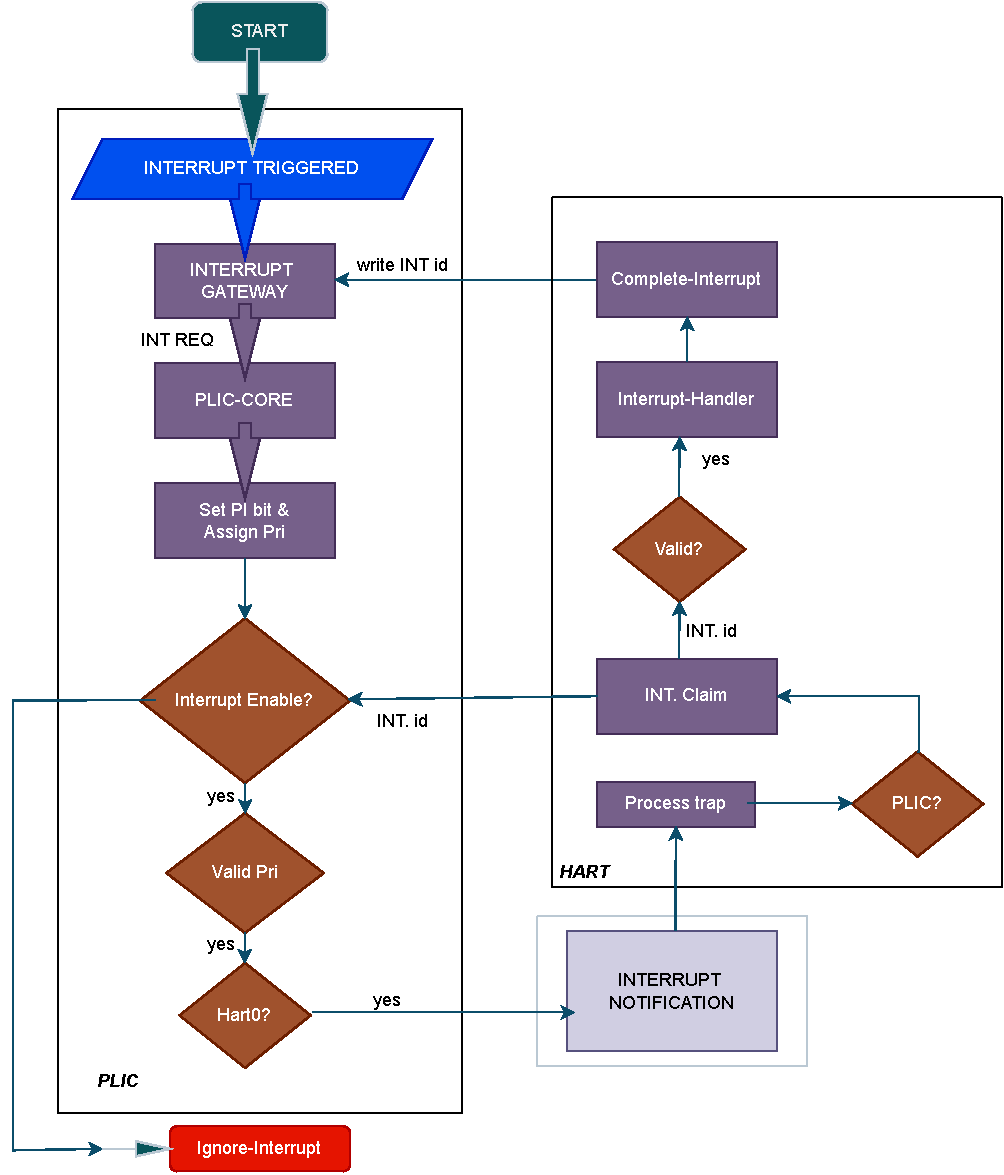
\includegraphics[width = 1\textwidth]{./shaheer_figures/fig_1.pdf}
		\rule{35em}{2pt}
	\caption{Interrupt Controller Overview}
	\label{fig:Structure of INT. controller}
\end{figure}

The PLIC in our case has finite interrupt sources. Some of these will be exposed at the top level via the GPIO pins. Other Interrupt sources are muxed with GPIO pins. They can be used by configuring pinmux registers. If pinmux value is zero, all the pins are GPIO configured. And if one pin goes to the I2C. The source of interrupts for PLIC are the devices connected to the SoC (GPIO, UART, I2C, etc...). As per the RISC-V specification these are termed as global interrupt sources. Global interrupt sources can take many forms, including level-triggered and edge-triggered. In our case, all the interrupts will be positive edge triggered. Our concept will be more clear by looking onto the above fig.

\section{Design Management Challanges}

\subsection{Design Flexibility and Complexity}

\maketitle
\begin{itemize}
    \item  Potentially hundreds and even thousands of registers 
in Memory Mapped Management Interface.

\item Interface Complexity discourages design changes.
\item  Documentation is time-consuming and error-prone.

\end{itemize}

\subsection{Interface Design Goals}

\maketitle
\begin{itemize}
\item Keep memory map as small as possible.
\item  Maintain an intuitive, logical arrangement of registers.
\item  Avoid need for manual maintenance of interface code.

\end{itemize}

\section{Design Management Solutions}

\subsection{Dynamic Memory Map}

\maketitle
\begin{itemize}
    \item   Easily adapt to wide range of parameters.
\item  Automate practical register arrangement.
\item  Automate documentation of memory map.

\end{itemize}

\subsection{No. of Registers}
\maketitle
\begin{itemize}
    \item Re-Use Read ID register as “Interrupt Claim”.
\item  Re-Use Write ID register as “Interrupt Complete”.

\end{itemize}

\section{PLIC Design Goals}


\maketitle
\begin{itemize}
    \item Easy integration with external 
bus interfaces.
\item  Support user defined number 
of Interrupt Sources and 
Targets.
\item Enabling and disabling of 
individual interrupt sources per 
target.
\item Full Priority Level and Priority 
Threshold support.
\item  Low latency handling of 
queued interrupt requests.

\item Programmable depth queue of 
pending interrupts.

\end{itemize}


